\section{Experimentación}

Presentaremos en esta sección la experimentación y discusión juntas, para cada experimento. Primero daremos una breve descripción de la instancia experimental, seguido de lo que esperamos observar, es decir, nuestra hipótesis. A continuación mostraremos los 
resultados obtenidos y nuestro análisis respecto a por qué obtuvimos dichos resultados.

\subsection{Metodología en la generación de instancias}

Para la creación de instancias de prueba, por una cuestión de practicidad, y para evitar sesgar los experimentos, decidimos utilizar instancias generadas aleatoriamente utilizando numpy. Todo el código de generación de datos, así como de corrida de tests, y las instancias utilizadas para la experimentación, se encuentran en la carpeta experimentos. En términos de las distribuciones utilizadas, en cada uno de los experimentos explicaremos las particularidades de la elección de distribución, pero aquí presentamos una tabla mostrando la distribución utilizada para la generación de los parámetros de las sanguijuelas:

\begin{center}
\begin{tabular}{l | l | l | l | l | l | l}
Experimento & Instancia & \#Sanguijuelas & X & Y & Radio & Temperatura\\ \hline
$1$ & $1$ & $50$ & $\mathcal{U}(45, 55)$ & $\mathcal{U}(45, 55)$ & $|\mathcal{N}(0.5, 10)|$ & $\mathcal{E}(1/100)$\\ \hline
$1$ & $2$ & $50$ & $\mathcal{U}(0, 100)$ & $\mathcal{U}(0, 100)$ & $|\mathcal{N}(2, 100)|$ & $\mathcal{E}(1/100)$\\ \hline
$1$ & $3$ & $50$ & $\mathcal{U}(0, 100)$ & $\mathcal{U}(0, 100)$ & $|\mathcal{N}(0.1, 10)|$ & $\mathcal{E}(1/300)$\\ \hline
$2$ & $1$ & $50$ & $\mathcal{U}(0, 100)$ & $\mathcal{U}(0, 100)$ & $\mathcal{U}(0, 10)$ & $\mathcal{E}(1/300)$\\ \hline
$3$ & $1$ & $31$ & Explicado & Explicado & Explicado & $\mathcal{E}(1/300)$\\ \hline
\end{tabular}
\end{center}

Todas las instancias son de $100x100$. En el caso del experimento 3 tomamos $h = 1$ para simplificar la generación de instancias, mientras que en los otros casos utilizamos

$$h \in \{0.5, 0.8, 1.0, 1.25, 2.0, 2.5, 4.0, 5.0, 6.25, 10.0, 12.5\}$$

Explicaremos más en profundidad estas decisiones en las subsecciones correspondientes. La elección de los valores de $h$ fue una tarea complicada: la restricción de $h | a \wedge h | b$ restringe ampliamente el conjunto de valores; fuera de eso, utilizar valores de granularidad demasiado pequeños aumenta demasiado el costo computacional, como veremos más adelante. Encontramos que intentar correr las instancias con un $h < 0.5$ elevaba demasiado el costo temporal de resolver el problema, por lo que utilizamos este valor como punto de comienzo.

\subsection{Experimento 1: variación de la temperatura en función de la granularidad}

Para este experimento, nos planteamos como objetivo mostrar que la matriz final de temperaturas es dependiente de la granularidad elegida para la instancia. Desde el punto de vista algorítmico, notemos que la granularidad impacta en las sanguijuelas que terminan determinando la temperatura inicial en los puntos: si una sanguijuela es lo suficientemente chica y está ubicada de forma tal que su radio no llega a impactar en el punto de la discretización más cercano, no será considerada como parte de la matriz. El experimento que ideamos consiste en crear una instancia donde todas las sanguijuelas estén muy cercanas al punto crítico, con radios lo suficientemente pequeños como para que el efecto que mencionamos antes logre aparecer. Tras un largo proceso de prueba y error, determinamos que las distribuciones mencionadas anteriormente eran las que mejor modelaban la idea intuitiva que estábamos buscando probar. En particular, la elección de una distribución exponencial se debe a que buscamos que las sanguijuelas tengan valores relativamente pequeños para que borrarlas logre mostrarnos un cambio concreto en la temperatura del punto crítico. Para todos los casos del experimento 1 utilizamos el método de eliminación gausiana para obtener las matrices de temperatura correspondientes.

Intuitivamente esperábamos que la temperatura en el punto crítico fuera aumentando a medida que achicásemos el $h$: suponíamos que aumentar la granularidad forzosamente iba a resultar en que la mayor temperatura de las sanguijuelas cercanas al centro tomase relevancia en el punto crítico e iba a hacer que la temperatura del mismo subiese, mientras que tener una menor granularidad debía hacer que cada vez más sanguijuelas se perdieran en la discretización y forzaría a que las sanguijuelas mejor posicionadas para los nuevos valores de $h$ dominen la temperatura en el punto crítico. De las instancias que corrimos, creemos que el gráfico \ref{fig:exp11} es ampliamente representativo.

\begin{figure}[h]
    \centering
    \includegraphics[width=0.685\textwidth]{experimento 1-1}
    \caption{Variación de la temperatura en función de la granularidad para la primera instancia}
    \label{fig:exp11}
\end{figure}

Es fácil observar que la temperatura del punto critico se estabiliza a medida que aumenta la granularidad, y tiende a ser más bien caótico a medida que aumentamos el valor de h, es decir, disminuimos la granularidad. A diferencia de lo que esperábamos, la temperatura con mayor granularidad no es la mayor de las obtenidas, encontramos que la granularidad de la discretización es más bien un parámetro de regulación para la precisión de la solución: cuanta mayor granularidad, más difícil es que las sanguijuelas que aparezcan cambien sustancialmente la temperatura del punto crítico, ya que un $h$ más pequeño implica que los radios de las sanguijuelas que quedan por descubrir son lo suficientemente chicos como para afectar pocos puntos, y la ecuación de calor parece "balancear" las temperaturas hacia los valores más frecuentes.

A modo de ayudar a la comprensión del experimento y la instancia contemplada, creamos una visualización del mapa de temperaturas generado por esta instancia particular, variando los valores de $h$:

\begin{figure}[h]
    \centering
    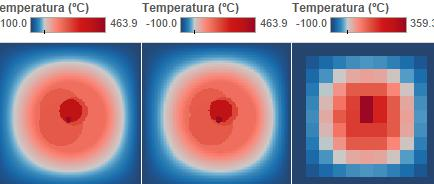
\includegraphics[width=0.685\textwidth]{Ejemplo Instancia 1}
    \caption{Mapa de calor para la instancia 1}
    \label{fig:exp11-vis}
\end{figure}

Observemos que a medida que disminuimos la granularidad, el borde con temperatura $-100$ºC comienza a tomar cada vez más relevancia dentro de la discretización, y colabora aun más que antes a reducir los valores de temperatura.

Para la segunda instancia pensamos en crear sanguijuelas de un radio grande, en comparación con la primera instancia, alejadas del punto critico. En este caso esperábamos, en principio, que la temperatura se mantuviese constante a medida que aumentamos la granularidad, pues las sanguijuelas son lo suficientemente grandes para no desaparecer dentro de la discretización y más aun, esperamos una variación pequeña de temperatura en relación al aumento del $h$. Observemos que en este caso cambiamos completamente la forma de generar las instancias de test, quitando restricciones en tanto a los valores de las sanguijuelas: el hecho de tomar distribución uniforme para las posiciones nos asegura la existencia de sanguijuelas en una variedad de puntos de la discretización, mientras que el radio normal nos da acceso a un panorama más variado en términos de los radios.

\begin{figure}[h]
    \centering
    \includegraphics[width=0.685\textwidth]{experimento 1-2}
    \caption{Variación de la temperatura en función de la granularidad para la segunda instancia}
    \label{fig:exp12}
\end{figure}

Observemos, en \ref{fig:exp12}, que efectivamente, la amplitud de temperatura es baja, menor a $5$ºC, confirmando nuestra hipótesis sobre la variación de la temperatura a lo largo del aumento de granularidad. Una vez más encontramos que el algoritmo converge a una solución a partir de cierto $h$ y se mantiene estable, aunque la diferencia en este caso es que el $h$ viene antes que en la instancia 1. Una vez más, proveemos una visualización de la clase generada para la instancia 2:

\begin{figure}[h]
    \centering
    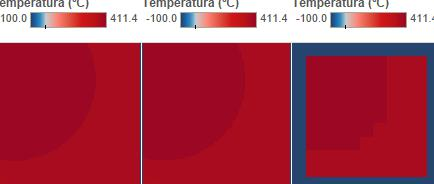
\includegraphics[width=0.685\textwidth]{Ejemplo Instancia 2}
    \caption{Mapa de calor para la instancia 2}
    \label{fig:exp12-vis}
\end{figure}


Como tercera instancia, nos planteamos ver qué sucede con las sanguijuelas más pequeñas al estar alejadas del centro. Para esto, generamos instancias con las distribuciones mencionadas anteriormente, pero observemos que en este caso tomamos la temperatura como una variable exponencial de esperanza $300$, es decir, tomamos valores de temperatura mucho más altos. Nuestro análisis de los casos anteriores nos induce a pensar que las sanguijuelas suficientemente peque\~nas no tendrán tanta relevancia en la temperatura del punto critico. Esto es porque, al afectar pocos puntos de la discretizaci\'on, la ecuación de calor compensa esos valores al alejarse de la posición de las sanguijuelas. 

\begin{figure}[h]
    \centering
    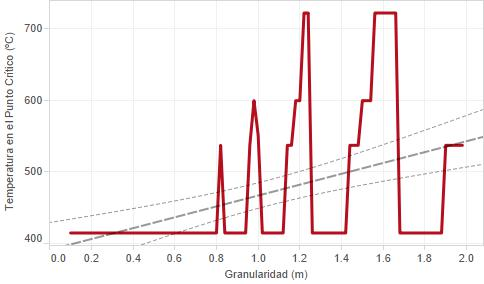
\includegraphics[width=0.685\textwidth]{experimento 1-3}
    \caption{Variación de la temperatura en función de la granularidad para la tercera instancia}
    \label{fig:exp13}
\end{figure}

En el gráfico podemos observar que la temperatura solo varia, para una granularidad muy baja, en el orden de los $20$ºC. Sin embargo, a diferencia de los casos anteriores, encontramos que la temperatura se estabiliza a valores cada vez mas bajos al aumentar la granularidad. Para explicar este comportamiento vamos a analizar el mapa de calor de la instancia 3.

\begin{figure}[h]
    \centering
    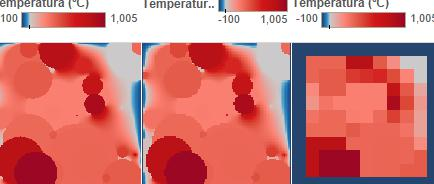
\includegraphics[width=0.685\textwidth]{Ejemplo Instancia 3}
    \caption{Mapa de calor para la instancia 3}
    \label{fig:exp13-vis}
\end{figure}

Podemos observar que, a medida que aumenta la granularidad, la disipación de temperatura aumenta. En particular, nos concentramos en las sanguijuelas de mayor temperatura. Vemos que, en el mapa de mayor granularidad, parece que los altos valores de temperatura se limitan al área cubierta por las mismas, mientras que la temperatura desciende drásticamente al salir del radio. Se puede, sin embargo, observar áreas de calor entre dos sanguijuelas relativamente cercanas, donde la función de disipación debe disipar calor en dos direcciones contrarias. Observado esto, solo podemos concluir que las sanguijuelas de mayor temperatura están demasiado alejadas entre si, por lo que las altas temperaturas se pierden automáticamente en la ecuación.

%%aca hay que agregar que pasaria si experimentaramos con lu

\subsection{Experimento 2: análisis del tiempo de computo en función de la granularidad}

\begin{figure}[H]
    \centering
    \includegraphics[width=0.685\textwidth]{experimento 2-1}
    \caption{Comparación entre EG y LU}
    \label{fig:exp21}
\end{figure}

\subsection{Experimento 3: comparación entre algoritmos para eliminación de sanguijuelas}%entre algoritmos para salvarnos la vida quedaba mas gracioso

En este experimento nos enfocamos en analizar las diferencias entre los algoritmos de eliminación de sanguijuelas, a los que llamaremos eliminación simple y eliminación con Sherman-Morrison.

Basados en los tests de correctitud, podemos afirmar que ambos algoritmos tienen el mismo comportamiento cualitativo. Es decir, ambos devuelven la misma solución. Por esto, el enfoque de este experimento es el análisis temporal de los experimentos. 

Antes de establecer hipótesis alguna, vamos a hacer un breve análisis del comportamiento esperado de cada algoritmo. 

\begin{figure}[H]
    \centering
    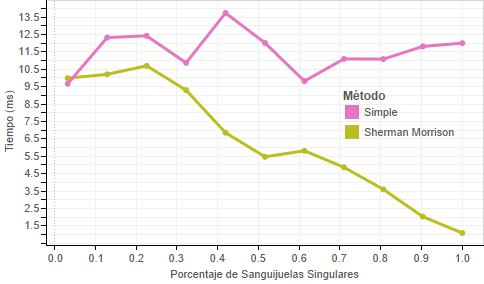
\includegraphics[width=0.685\textwidth]{experimento 3-1}
    \caption{Comparación entre SM y el método simple}
    \label{fig:exp31}
\end{figure}
